\documentclass[tikz,border=4pt]{standalone}
% Estilo común de los diagramas de bloques (se usa con \input en cada standalone)
\usepackage[defaultsans,scale=0.92]{lato}
\usepackage{libertinust1math}
\usepackage{xcolor,amsmath}
\usepackage{tikz}
\usetikzlibrary{positioning,arrows.meta,calc,shapes.geometric}
\usepackage{../../notacion}
\definecolor{ctrlazul}{HTML}{1E5AA8}\definecolor{ctrlnoche}{HTML}{14213D}
\definecolor{ctrlcoral}{HTML}{D1495B}\definecolor{ctrlverde}{HTML}{2A9D8F}
\definecolor{ctrlambar}{HTML}{E09F3E}\definecolor{ctrlgris}{HTML}{5C677D}
\definecolor{ctrlvioleta}{HTML}{6C4AB6}\definecolor{ctrlteal}{HTML}{0F7173}
\tikzset{
  >={Stealth[length=2.4mm]}, every node/.style={font=\small},
  bloque/.style={draw=ctrlnoche,fill=ctrlazul!7,thick,rounded corners=1.5pt,minimum height=9mm,minimum width=13mm,inner sep=4pt},
  suma/.style={draw=ctrlnoche,thick,circle,inner sep=0pt,minimum size=6mm},
  senal/.style={->,thick,draw=ctrlnoche},
  rot/.style={font=\footnotesize,text=ctrlgris},
}

\begin{document}
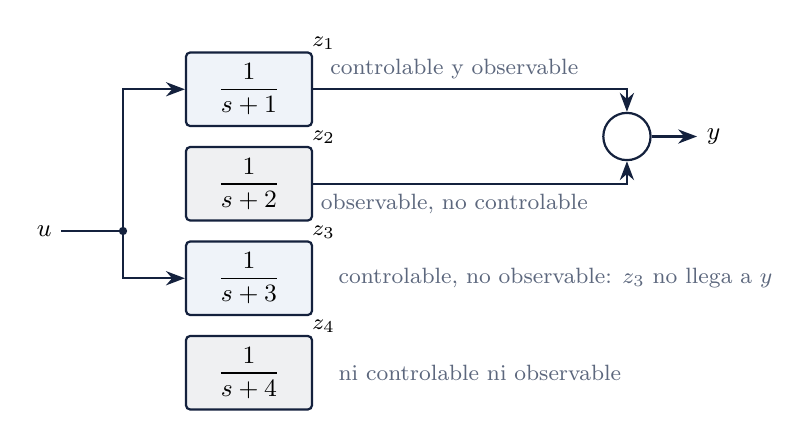
\begin{tikzpicture}[b/.style={bloque,minimum width=16mm}]
  \node (u) at (0,0) {$u$};
  \coordinate (n) at (1.0,0);
  \node[b] (z1) at (2.6, 1.8) {$\dfrac{1}{s+1}$};
  \node[b,fill=ctrlgris!10] (z2) at (2.6, 0.6) {$\dfrac{1}{s+2}$};
  \node[b] (z3) at (2.6,-0.6) {$\dfrac{1}{s+3}$};
  \node[b,fill=ctrlgris!10] (z4) at (2.6,-1.8) {$\dfrac{1}{s+4}$};
  \node[suma] (S) at (7.4,1.2) {};
  \node (y) at (8.5,1.2) {$y$};
  \draw[thick,draw=ctrlnoche] (u)--(n); \fill[ctrlnoche] (n) circle (1.5pt);
  \draw[senal] (n)|-(z1); \draw[senal] (n)|-(z3);
  \draw[senal] (z1.east)--node[above,pos=0.45,rot]{controlable y observable}(7.4,1.8)--(S);
  \draw[senal] (z2.east)--node[below,pos=0.45,rot]{observable, no controlable}(7.4,0.6)--(S);
  \draw[senal] (S)--(y);
  \node[rot,anchor=west] at ($(z3.east)+(2mm,0)$) {controlable, no observable: $z_3$ no llega a $y$};
  \node[rot,anchor=west] at ($(z4.east)+(2mm,0)$) {ni controlable ni observable};
  \foreach \i in {1,...,4} \node[font=\footnotesize,anchor=south east] at ($(z\i.north east)+(4mm,-1mm)$) {$z_\i$};
\end{tikzpicture}
\end{document}
